\documentclass[a4 paper]{article}
% Set target color model to RGB
\usepackage[inner=2.0cm,outer=2.0cm,top=1.7cm,bottom=1.4cm]{geometry}
\usepackage{setspace}
\usepackage[rgb]{xcolor}
\usepackage{verbatim}
\usepackage{subcaption}
\usepackage{amsgen,amsmath,amstext,amsbsy,amsopn,tikz,amssymb,tkz-linknodes}
\usepackage{fancyhdr}
\usepackage[colorlinks=true, urlcolor=blue,  linkcolor=blue, citecolor=blue]{hyperref}
\usepackage[colorinlistoftodos]{todonotes}
\usepackage{rotating}
\usepackage{floatrow}
\usepackage{amsmath}
\usepackage{xspace}
% \usepackage{subfig}
\usepackage{enumitem}
\usepackage{bbm}
% for placing picture here
% \usepackage[section]{placeins}

\usepackage{booktabs}
\newcommand{\ra}[1]{\renewcommand{\arraystretch}{#1}}

\newtheorem{thm}{Theorem}[section]
\newtheorem{prop}[thm]{Proposition}
\newtheorem{lem}[thm]{Lemma}
\newtheorem{cor}[thm]{Corollary}
\newtheorem{defn}[thm]{Definition}
\newtheorem{rem}[thm]{Remark}
\numberwithin{equation}{section}

\newcommand{\homework}[6]{
   \pagestyle{myheadings}
   \thispagestyle{plain}
   \newpage
   \setcounter{page}{1}
   \noindent
   \begin{center}
   \framebox{
      \vbox{\vspace{2mm}
    \hbox to 6.28in { {\bf COL774:~Machine Learning \hfill { #2}} }
       \vspace{6mm}
       \hbox to 6.28in { {\LARGE \hfill #1  \hfill} }
       \vspace{6mm}
       \hbox to 6.28in {\bf {Entry Number: {\rm #4} \hfill Name: {\rm #5} } }
       % \hbox to 6.28in { {\it TA: #4  \hfill #6}}
      \vspace{2mm}}
   }
   \end{center}
   \markboth{#1}{#1}
   \vspace*{4mm}
}

% \newcommand{\problem}[2]{~\\\fbox{\textbf{Problem #1}}\hfill (#2 points)\newline\newline}
% \newcommand{\subproblem}[1]{~\newline\textbf{(#1)}}
% \newcommand{\D}{\mathcal{D}}
% \newcommand{\Hy}{\mathcal{H}}
% \newcommand{\VS}{\textrm{VS}}
% \newcommand{\solution}{~\newline\textbf{\textit{(Solution)}} }

% \newcommand{\bbF}{\mathbb{F}}
% \newcommand{\bbX}{\mathbb{X}}
% \newcommand{\bI}{\mathbf{I}}
% \newcommand{\bX}{\mathbf{X}}
% \newcommand{\bY}{\mathbf{Y}}
% \newcommand{\bepsilon}{\boldsymbol{\epsilon}}
% \newcommand{\balpha}{\boldsymbol{\alpha}}
% \newcommand{\bbeta}{\boldsymbol{\beta}}
% \newcommand{\0}{\mathbf{0}}

\begin{document}
\homework{Assignment 1 Report}{Date: February 12, 2019}{}{\bf 2016CS10363}{\bf Manish Tanwar}{NetId(s)}

\section{Linear Regression:}
\textbf{Note:} I have normalized the data and calculated the parameters back for original data.

\subsubsection*{(a):}

\begin{itemize}
	\item Learning Rate = 0.5
	\item \textbf{Stopping Criteria:}
$$ \hspace*{3.25cm} \big| \theta_j^{(t+1)} - \theta_j^{(t)} \big| < \epsilon \quad \quad \forall j \in {1,2...n} \hspace*{1.65cm} (\text{for a sufficiently small } \epsilon \text{ (took } \epsilon = 10^{-4}))$$
	\item {Parameters (Calculated for original(unnormalized) data):}
	$$ \hspace*{-3.75cm} \theta = 
	\begin{bmatrix}
		\theta_0 \\  \theta_1 \\
	\end{bmatrix}
	= 
	\begin{bmatrix}
		0.990289 \\
		0.000778
	\end{bmatrix} $$

\end{itemize}

\subsubsection*{(b):}
\begin{figure}[H]
	\centering
	% \hspace*{-0.9in} % width=100mm
	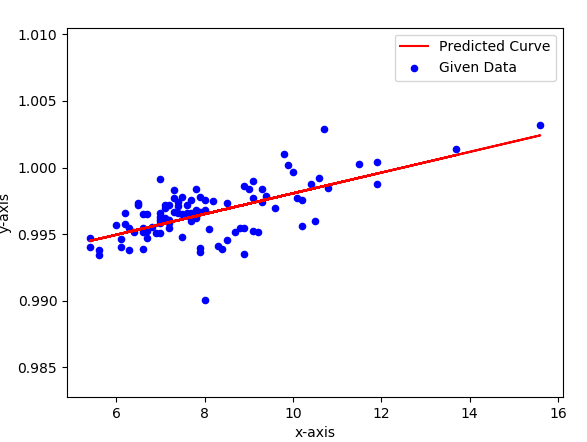
\includegraphics[width = 90mm]{./Plots/1b.png}
	\caption{Linear Regression : Data Points and Hypothesis Function Plot}
  	\label{fig9}
\end{figure}

\subsubsection*{(c): \hspace*{8.3cm} (d):}

\begin{figure}[H]
	\centering
    \begin{floatrow}
	\hspace*{-0.4in}
      \ffigbox[\FBwidth]{\caption{Linear Regression : 3D mesh}\label{fig12}}{%
      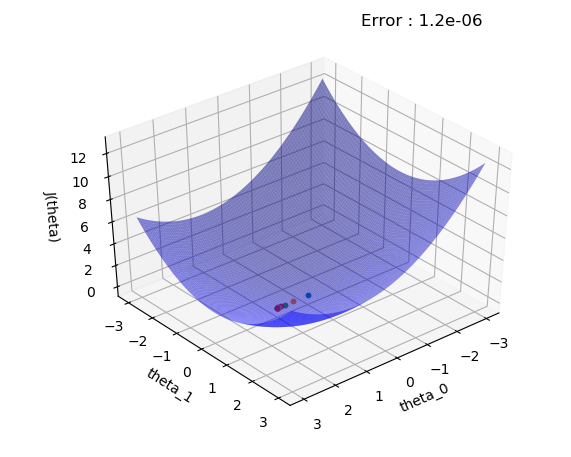
\includegraphics[width=90mm]{./Plots/1c.png}
      }
      \ffigbox[\FBwidth]{\caption{Linear Regression : Contours}\label{fig13}}{%
		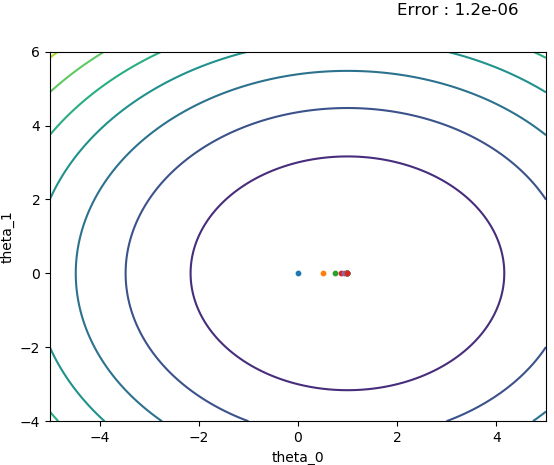
\includegraphics[width=90mm]{./Plots/1d.png}
      }
    \end{floatrow}
\end{figure}

\subsubsection*{(e) Observations:}
% η = {0.1, 0.5, 0.9, 1.3, 1.7, 2.1, 2.5}
On plotting the contours figures for various values of Learning Rate($\eta$), we get the following observations:
\begin{itemize}
	\item For $\eta \in \{0.1, 0.5, 0.9\}$, the error function converges to the minima.
	\item For $\eta \in \{1.3, 1.7\}$, the error function overshoots to the other side of the minima and toggles around the minima and finally converges.
	\item For $\eta \in \{2.1, 2.5\}$, the error fuction diverges from the minima.
	\item The number of iterations required decreases as we increase the learning rate($\eta$), but after a certain value when the error function overshoots it takes more iterations to converge and finally the error function diverges on large learning rates. 
\end{itemize}

% *********** 2 ***************
\section{Locally Weighted Linear Regression:}

\vspace*{-0.15cm}

\subsection*{(a) Linear Regression (unweighted):}
\vspace*{-0.1cm}
$$ \hspace*{-0.75cm} \theta = 
\begin{bmatrix}
	\theta_0 \\  \theta_1 \\
\end{bmatrix}
= 
\begin{bmatrix}
	0.327680 \\
	0.175316
\end{bmatrix} $$

\vspace*{-0.2cm}
\begin{figure}[H]
	\centering
	% \hspace*{-0.9in} % width=100mm
	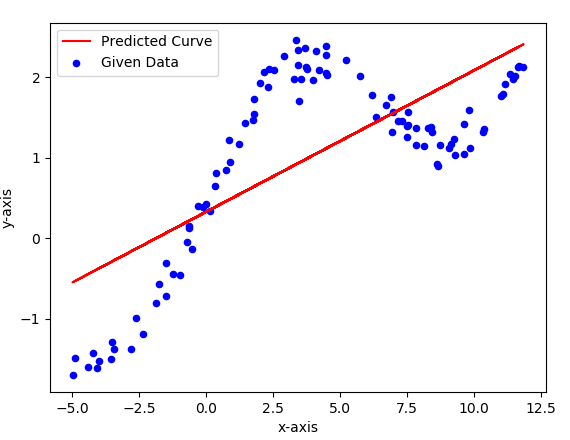
\includegraphics[width = 90mm]{./Plots/2a.png}
	\caption{Linear Regressin Plot (Underfitting)}
  	\label{fig1}
\end{figure}

Linear Regression(unweighted) is not a good fit for the data as shown in the Figure 1(underfitting).

\subsection*{(b) Locally Weighted Linear Regression:}
\vspace*{0.3cm}
$$ \hspace*{-2.5cm}\text{Weights}: \hspace*{1.9cm} w^{(i)} = \exp\left(-\frac{(x-x^{(i)})^2}{2\tau^2}\right) \quad \quad \quad (\text{where } \tau = \text{Bandwidth Parameter}) $$

$$ \hspace*{-2.7cm} \text{Error Function: } \hspace*{0.9cm} J(\theta) = \frac{1}{2m} (X\theta - Y)^TW(X\theta - Y) \hspace*{1cm} (\text{where } W = diag(w^{(i)}) \hspace*{0.5mm}) $$


$$ \hspace*{-5.8cm} \text{Minima:} \hspace*{2.3cm} \nabla_{\theta}J(\theta) = 0 \quad \Rightarrow \quad \theta = (X^TWX)^{-1}X^TWY $$

% \newpage
\vspace*{0.1cm}
\hspace*{-0.2cm}
\textbf{Plots:}

\begin{figure}[H]
	\centering
	% \hspace*{-0.9in} % width=100mm
	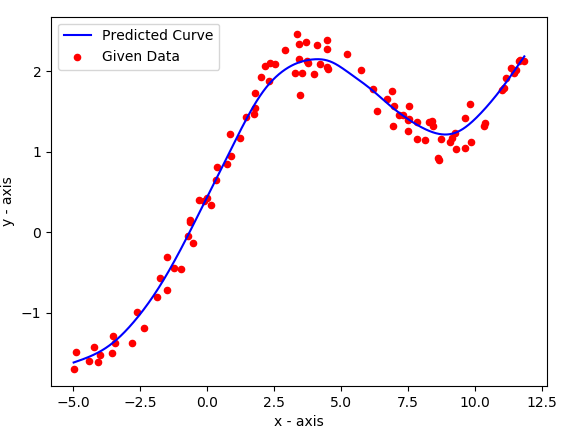
\includegraphics[width = 90mm]{./Plots/2b(08).png}
	\caption{Locally Weighted Linear Regressin Plot ($\tau = 0.8$)}
  	\label{fig2}
\end{figure}

\vspace*{-0.5cm}
\subsection*{(c) Plots on Varying Bandwidth Parameter($\tau$)}

\vspace*{-0.7cm}
\begin{figure}[H]
	\centering
    \begin{floatrow}
	\hspace*{-0.4in}
      \ffigbox[\FBwidth]{\caption{$\tau = 0.1$}\label{fig3}}{%
      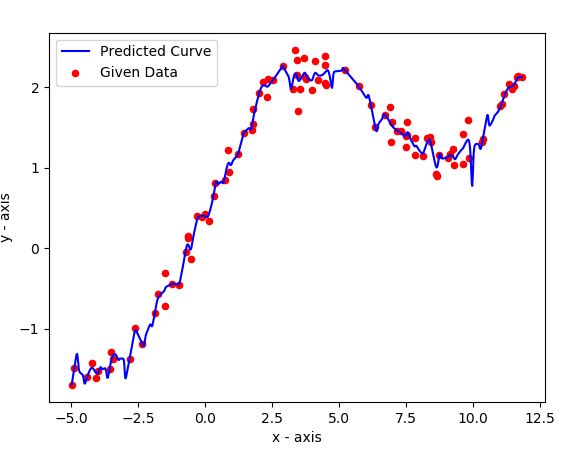
\includegraphics[width=90mm]{./Plots/2b(01).png}
      }
      \ffigbox[\FBwidth]{\caption{$\tau = 0.3$}\label{fig4}}{%
		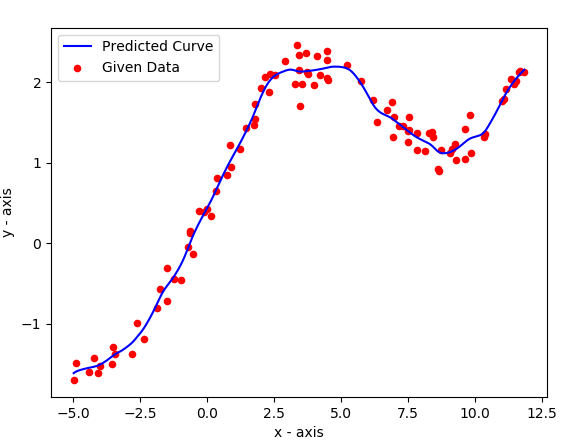
\includegraphics[width=90mm]{./Plots/2b(03).png}
      }
    \end{floatrow}
\end{figure}

\vspace*{-0.82cm}
\begin{figure}[H]
	\centering
    \begin{floatrow}
	\hspace*{-0.4in}
      \ffigbox[\FBwidth]{\caption{$\tau = 2$}\label{fig5}}{%
      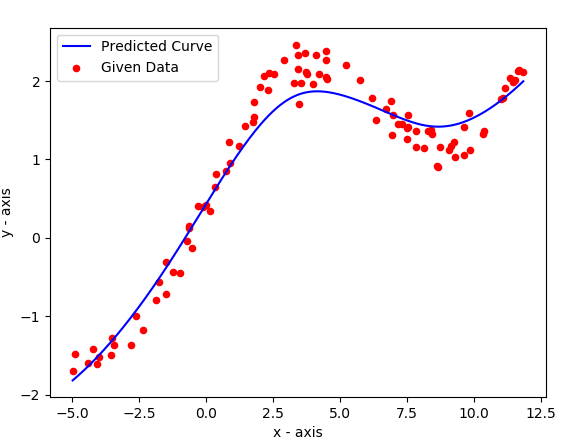
\includegraphics[width=90mm]{./Plots/2b(2).png}
      }
      \ffigbox[\FBwidth]{\caption{$\tau = 10$}\label{fig6}}{%
		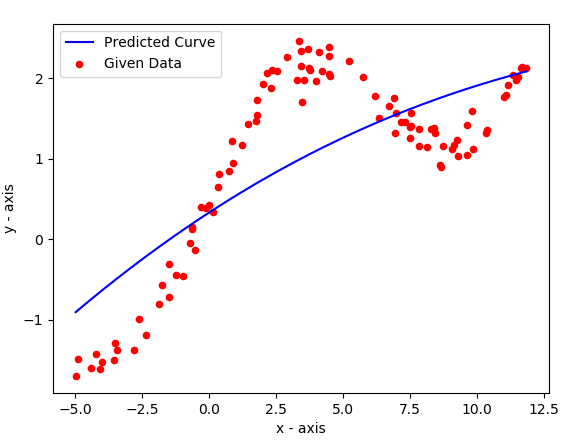
\includegraphics[width=90mm]{./Plots/2b(10).png}
      }
    \end{floatrow}
\end{figure}

\subsection*{Analysis:}
	
\begin{itemize}
	\item When Bandwidth Parameter($\tau$) is:
	\begin{itemize}
	\item \textbf{Too Small:} It results in \textbf{overfitting}.
	\item \textbf{Too Large:} It results in \textbf{underfitting}.
	\end{itemize}
	\item If $\tau$ is too small the model looks at really close data-points to the query data point $x$ which results in overfitting and if $\tau$ is too large it predicts the query data point based on giving all the data same weights(overgeneralization) which results in underfitting.
	\item $\tau = 0.8$ works the best in our case.
\end{itemize}

% *********** 3 ***************
\section{Logistic Regression:}
\vspace*{0.3cm}

$$ \hspace*{-4.3cm} \text{Log Likelihood:} \hspace*{0.8cm} LL(\theta) = \sum_{i=1}^{m} y^{(i)} log(h_{\theta}(x^{(i)})) + (1 - y^{(i)}) log(1-h_{\theta}(x^{(i)}))  $$

$$ \hspace*{0.7cm} \nabla_{\theta}LL(\theta) = X^T(Y - g(X\theta)) \hspace{2cm} (\text{where } g(x) = \frac{1}{1 + \exp(-x)}) $$

$$ \hspace*{-6.6cm} \text{Hessian Matrix: } \hspace*{0.9cm} H = \nabla_{\theta}^2LL(\theta) = -X^T D X \hspace*{2cm} $$
$$ \hspace*{4.6cm} (\text{where } D = diag( \hspace*{0.5mm} g(x^{(i)T}\theta) (1 - g(x^{(i)T}\theta)) \hspace*{0.5mm}) $$

\vspace*{0.2cm}
\hspace*{-0.2cm} 
\textbf{Newton's Method:}
$$\hspace*{-2.65cm} \theta^{(t+1)} = \theta^{(t)} - H^{-1}\nabla_{\theta}LL(\theta)\big|_{\theta_{t}}$$

\vspace*{0.2cm}
\hspace*{-0.2cm} 
\textbf{Stopping Criteria:}
$$ \hspace*{3.25cm} \big| \theta_j^{(t+1)} - \theta_j^{(t)} \big| < \epsilon \quad \quad \forall j \in {1,2...n} \hspace*{1.65cm} (\text{for a sufficiently small } \epsilon \text{ (took } \epsilon = 10^{-8}))$$

\hspace*{-0.2cm} 
\textbf{Resulting Parameters:}
$$ \hspace*{-3.75cm} \theta = 
\begin{bmatrix}
	\theta_0 \\  \theta_1 \\ \theta_2 \\
\end{bmatrix}
= 
\begin{bmatrix}
	0.223295 \\  1.962616 \\ -1.964861\\
\end{bmatrix} $$

\hspace*{-0.2cm} 
Decision Boundary is the straight line boundary separating the region where $h_\theta(x) \geq 0.5 \hspace*{0.5mm} (\text{class } y=1)$ from
where $h_\theta(x) \leq 0.5 \hspace*{0.5mm} (\text{class } y=0)$.

\newpage
% \vspace*{0.5cm}
\hspace*{-0.2cm} 
\textbf{Plot:}
\begin{figure}[H]
	\centering
	% \hspace*{-0.9in} % width=100mm
	  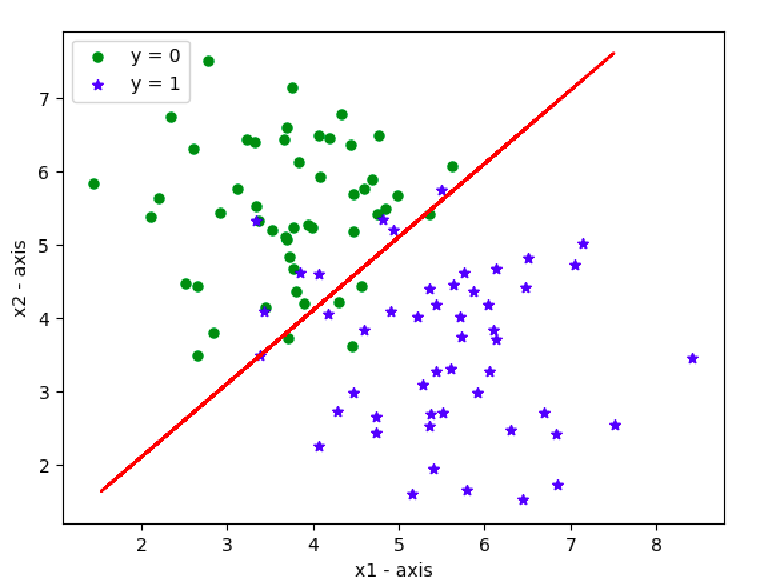
\includegraphics[width = 90mm]{./Plots/3.png}
	  \caption{Logistic Regression : Given data and Linear Separator}
  	\label{fig7}
\end{figure}

\section{Gaussian Discrmimant Analysis:}

\subsection*{(a):}

$$ \phi = \frac{1}{m} \sum_{i=1}^{m} \mathbbm{1}\{y^{(i)}=1\} \hspace*{0.5cm}
\mu_0 = \frac{\sum_{i=1}^{m} \mathbbm{1}\{y^{(i)}=0\} x^{(i)}}{\sum_{i=1}^{m} \mathbbm{1}\{y^{(i)}=0\}} \hspace*{0.5cm}
\mu_1 = \frac{\sum_{i=1}^{m} \mathbbm{1}\{y^{(i)}=1\} x^{(i)}}{\sum_{i=1}^{m} \mathbbm{1}\{y^{(i)}=1\}}  $$

$$ \Sigma = \frac{1}{m} \sum_{i=1}^{m} (x^{(i)}-\mu_{y^{(i)}})(x^{(i)}-\mu_{y^{(i)}})^{T}$$

$$ \text{which can be written as:} \hspace*{1cm} \Sigma = \frac{1}{m} W^T W \hspace*{2cm} (\text{where } W = X - Y\mu_1^T - (1-Y)\mu_0^T) $$

\textbf{Resulting Parameters:}
$$ \phi = 0.5 \quad \quad
\mu_0 = 
\begin{bmatrix}
	98.38 \\ 429.66\\
\end{bmatrix} \quad \quad
\mu_1 = 
\begin{bmatrix}
	137.46 \\ 366.62 \\ 
\end{bmatrix} \quad \quad
\Sigma = 
\begin{bmatrix}
	287.482 & -26.748 \\ 
    -26.748 & 1123.25  \\
\end{bmatrix} $$

\subsection*{(b) \& (c):}
\subsubsection*{(i) Linear Boundary Equation:}

	$$ 2(\mu_1^T - \mu_0^T\Sigma^{-1})x + \mu_0^T \Sigma^{-1} \mu_0 - \mu_1^T \Sigma^{-1} \mu_1 - 2\log\left(\frac{1-\phi}{\phi}\right) = 0$$

\vspace*{-0.5cm}
\subsubsection*{(ii) Plot:}
\vspace*{-0.7cm}
\begin{figure}[H]
	\centering
	% \hspace*{-0.9in} % width=100mm
	  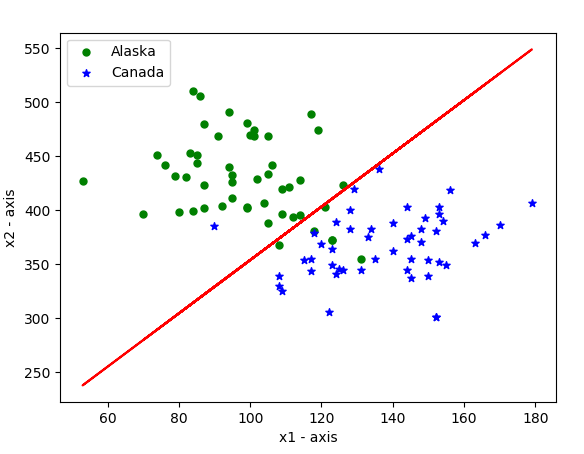
\includegraphics[width = 90mm]{./Plots/4a.png}
	  \caption{GDA : Given data and Linear Separator}
  	\label{fig8}
\end{figure}

\subsection*{(d):}
$$ \phi = \frac{1}{m} \sum_{i=1}^{m} \mathbbm{1}\{y^{(i)}=1\} \hspace*{0.5cm}
\mu_0 = \frac{\sum_{i=1}^{m} \mathbbm{1}\{y^{(i)}=0\} x^{(i)}}{\sum_{i=1}^{m} \mathbbm{1}\{y^{(i)}=0\}} \hspace*{0.5cm}
\mu_1 = \frac{\sum_{i=1}^{m} \mathbbm{1}\{y^{(i)}=1\} x^{(i)}}{\sum_{i=1}^{m} \mathbbm{1}\{y^{(i)}=1\}}  $$

$$ \hspace*{1cm} \Sigma_0 = (X-\mu_0^{ext})^Tdiag(y^{(i)})(X-\mu_0^{ext}) \hspace*{0.5cm} (\text{where } \mu_0^{ext} \text{ is } m \times n \text{ matrix with each row}= \mu_0^T) $$

\vspace*{0.5cm}
\textbf{Resulting Parameters:}
$$ \phi = 0.5 \quad \quad
\mu_0 = 
\begin{bmatrix}
	98.38 \\ 429.66\\
\end{bmatrix} \quad \quad
\mu_1 = 
\begin{bmatrix}
	137.46 \\ 366.62 \\ 
\end{bmatrix} $$
$$\Sigma_0 = 
\begin{bmatrix}
	255.3956 & -184.3308 \\ 
   -184.3308 & 1371.1044 \\
\end{bmatrix} \quad \quad \quad 
\Sigma_1 = 
\begin{bmatrix}
	319.5684 & 130.8348 \\
 	130.8348 & 875.3956 \\
\end{bmatrix}$$

\subsection*{(e):}

\subsubsection*{(i) Quadratic Boundary Equation:}

	$$ (x-\mu_1)^T \Sigma_1^{-1} (x-\mu_1) - (x-\mu_0)^T \Sigma_0^{-1} (x-\mu_0) + \log \left(\frac{|\Sigma_1|}{|\Sigma_0|} \frac{(1-\phi)^2}{\phi^2} \right) = 0$$

\subsubsection*{(ii) Plot:}

\begin{figure}[H]
	\centering
	% \hspace*{-0.9in} % width=100mm
	  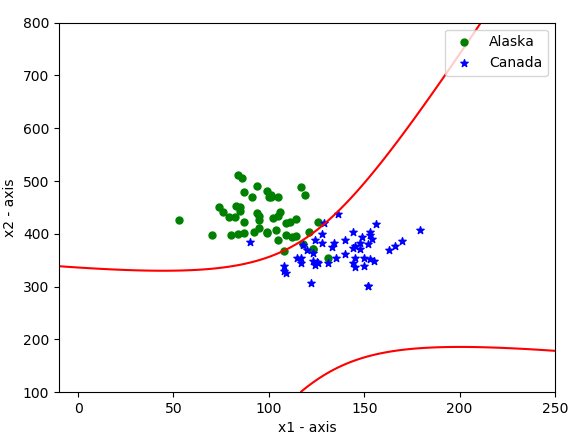
\includegraphics[width = 90mm]{./Plots/4b.png}
	  \caption{GDA : Given data and Quadratic Separator}
  	\label{fig8}
\end{figure}

\subsection*{(f) Analysis:}
\begin{itemize}
	\item In our case both linear and hyperbolic boundaries separates the data to a fair extend.
	\item But hyperbola gives 3 classes(Area-1, Area-2, Area-3 as shown in Figure 12) in the graph: \\
	$$\text{Area-1 and Area-3} \quad \Rightarrow \quad y=0 $$ 
	$$\text{Area-2} \quad \Rightarrow \quad y=1 $$ 
	This classifier classifies Area-1 in $y=0$ class, which does not seem to be true in this case. This dataset does not contain any point in Area-1. \\
	Similarly ellipse and hyperbola are conics which won't be able to classify linearly separated data.  
	\item As we make stronger assumption in case of linear separator($\Sigma_0 = \Sigma_1$) which could not be true some times, so quadratic separator would perform better than the linear separtor in these type of the cases.
\end{itemize}
\end{document}